Quick overview of things you'll need to understand while keeping me consistent with the litterature:

\begin{enumerate}
    \item Upper/Lower $\rightarrow$ Dorsal/Ventral
    \item Front/Back  $\rightarrow$ Anterior/Posterior
    \item   $\rightarrow$
\end{enumerate}
\section{Drosophila Gastrulation in detail}
In 1975 Bownes et al. split the development of the fruit fly from fertilised egg to hatched larvae into 17 distinct events. \cite{bownes1975photographic} These
We will be looking at stages 5 through 7, lasting about 15 minutes. These are characterized by having the first mesoscopic morphogenetic movements.

The Drosophila morphogenesis consist of a series of interconnected localized cell movements. I will here present an abridged (The "Good Parts" Version) overview, roughly ordered in time:\\

[YYY] stor figur.\\

\begin{enumerate}
    \item Three independent invaginations happen
    \begin{enumerate}
        \item Two slanted furrows (symmetrically on the "port" and "starboard" side) form vertically\footnote{along the Dorsal/Venrral-axis} about 1/3 of the length from the Apical tip\cite{}. This will form the Cephalic Furrow, separating the what will become the head from what will become the body. 
        \item  On the Ventral side, a 8x60 cell\cite{} begins invagination, pulling in the surrounding mesoderm. This is done via anisotropic\cite{} apical constriction\cite{}.
        \item The YYY-proteins start signaling\cite{} and a 4-cell wide 10-cell radius\cite{} ring on the posterior tip starts isotropic apical constriction\cite{}.
    \end{enumerate}
    \item One the dorsal side, the amnioserosa utilizes the AP-(even-skip and YYY)-patterning\cite{} and starts the creation of 2 transverse folds of 4- and 6- cell width respectively, pulling the invaginating posterior away from the ventral surface.
    \item  A force (speculative: originating at the ventral furrow) moves the partly formed PMG halfway towards the anterior tip, stretching the germ band along with it.
    \item ...
    \item profit
\end{enumerate}




\section{Broken Bymmetries and Genetic Patterning}
% \section{Everything}
\subsection{Broken Symmetries}

Snak om snefnug?

Almost all animals [Citation needed] start as a single, isotropic shell of epithelial cells. This shell will 'turn in on itself' and begin developing the basis for organogenesis. This process is called gastrulation. As most animals are not spherically symmetric\footnote{haha din mor}, a number of symmetries need to be broken. 

The blastula cells lie in a closely packed sphere with a distinct inside and outside, giving rise to the well-defined Apical-Basal polarity (AB-polarity from here on).

YY off-equilibrium densities with the gradients. These are called morphogens and 
In a W for computational biology, the mechanics of morphogens where predicted by none other than Alan Turing

In general, most of the global large-scale cell migration seen during development of multicellular organisms stem from a handful of seemingly simple\footnote{albeit still not well understood} active single-cell actions \cite{walck2014cell}. These 'driving effects' are surprisingly under-understood with no paper claiming YYY without being disputed within the field. (This comes down to the fact, that experiments with living, moving cells are inherently intractable) Here is a list of the fundamental single-cell active forces that is undeniably happening, even if not essential for the final outcome:\footnote{As nature is remarkably resilient, there is clear and definite evidence of one action overtaking when another fails to deliver \cite{butler2009cell} \textbf{Rewrite}} 
\begin{outline}
    \1 Cell intercolation (Germ Band Extension)
    \1 Apical Constriction
    \1 Cell Shape Change
    \1 Proliferation
\end{outline}

We will quickly outline the main morphological features of the gastrulation cycle of the embryo:
\begin{outline}
    \1 Posterior Midgut (PMG)
    \1 Anterior Midgut (AMG)
    \1 Ventral Furrow
    \1 Dorsal Transverse Furrows
    \1 Cephalic Furrow
    \1 Germ Band
\end{outline}

\begin{figure}[H]
    \centering
    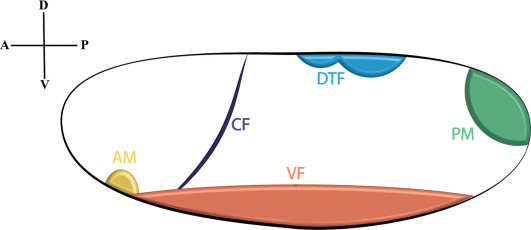
\includegraphics[width = 0.7\linewidth]{figures/morphogenic_events.jpg}
    \caption{Summary of the morphogenetic events mapped onto the blastoderm stage embryo. Taken from \cite{gheisari2020gastrulation}. The colored parts can be seen as the most morphogenetically active during embryogenesis}
    \label{fig:enter-label}
\end{figure}



Diffusion based concentration gradients along with the aforementioned polarities allow for spatially complex, precise and robust macro scale morphology changes.

\subsection{Genetic Patterning}
All multicellular organisms, will YYY need to go from the simple single cell to forming the complex body plans we all know and love. This complicated interplay between cells will 

Needs organization. Again, for humans and fruit fly alike, this is done via genetic patterning.\cite{veraksa2000developmental} 


\begin{table}[]
\begin{tabular}{llll}
Morphogen & \begin{tabular}[c]{@{}l@{}}Genetically patterned \\ transcription factor proteins\end{tabular} & Location at gastrulation & Vital for development of \\ \hline
Spätzle   & Twist \& Snail                                                                                 & Ventral                  & Mesoderm                 \\
Trunk     & Huckebein \& Tailless                                                                          & Posterior                & Endoderm (Midgut)   \\

YYY & Runt \& Even skipped & Germ Band & All of the above\\
YYY & Buttonhead \& Even skipped  & Cephalic furrow & Chephalic furrow\\

\end{tabular}
\end{table}

\noindent
Now, to shake it up, \textit{Twist} \& \textit{Snail}, which might remind you of the beetles,\footnote{The species \textit{Tribozium} for example\cite{sommer1994expression}} are vital for the early development of a surviving fruit fly.


During the development of our model, the data and ressources at \url{https://shiny.mdc-berlin.de/DVEX/} have been absolutely vital.

\section{How cells move}
Newtons first law of motion seems to prevent any internal movement

Of course cell motility is important 


Cytoskeleton

Important: Fundamentally different from Chemotaxis 

Main motor protein on our scale:  \textit{Myosin II} (driver of Apical constriction for example) 

Membrane tethers connecting local neighborhoods.

Anisotropic constricting at cell borders \url{https://www.youtube.com/watch?v=MO7x7R-m3Qk}


\begin{figure}[H]
    \centering
    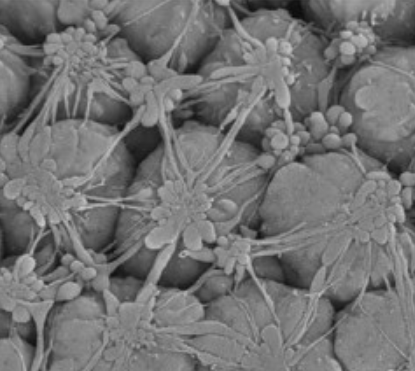
\includegraphics[width=0.6\linewidth]{chapters/Theory/figures/EM_constricting_proteins.png}
    \caption{Electron microscopy of Myosin II meshwork at ventral side. Taken from \cite{martin2010integration}}
    \label{fig:enter-label}
\end{figure}



\section{Previous attempts at simulation?}
\section{Overdamped dynamics}

\section{\textit{The Model}}
This all leads us to to our:


The model is built around simply simulating the movement of the center of mass of the cells (maybe nuclei?). This means that there is no simulated strains the


As described in \cite{} and \cite{}, the model we have been working with is defined by the intercellular poential:

\begin{equation}
    V_{ij}=e^{-r_{ij}}-A_{ij}e^{-r_{ij}/\beta}
\end{equation}

For all Voronoi neighbors.\\

A works as follows:
\begin{equation}
    A_{ij}=\sum_{n=1}^{3}\lambda_n A_n
\end{equation}
where we sometimes keep the constraint $\sum_{n=1}^{3}\lambda_n=1$ but more often t
